\documentclass[11pt,a4paper]{report}

\usepackage{algorithm}
\usepackage[noend]{algpseudocode}
\usepackage{algpseudocode}
\usepackage{amsmath}
\usepackage{amssymb}
\usepackage{booktabs}
\usepackage{dsfont}
\usepackage{enumitem}
\usepackage[a4paper]{geometry}
\usepackage{graphics}
\usepackage{graphicx}
\usepackage{hyperref}
\usepackage[utf8]{inputenc}
\usepackage{natbib}
\usepackage{parskip}
\usepackage{pgf-pie}
\usepackage{tabularx}
\usepackage{todonotes}
\usepackage{url}
\usepackage{xcolor}
\usepackage{xurl}

% Define nice pie chart colors
\definecolor{pie1}{HTML}{03045e}
\definecolor{pie2}{HTML}{023e8a}
\definecolor{pie3}{HTML}{0077b6}
\definecolor{pie4}{HTML}{0096c7}
\definecolor{pie5}{HTML}{00b4d8}
\definecolor{pie6}{HTML}{48cae4}
\definecolor{pie7}{HTML}{90e0ef}
\definecolor{pie8}{HTML}{ade8f4}
\definecolor{pie9}{HTML}{caf0f8}

\setlength{\marginparwidth}{2cm}
\hypersetup{
    colorlinks,
    citecolor=black,
    filecolor=black,
    linkcolor=black,
    urlcolor=black
}

% Set the line spacing between paragraphs
% \setlength{\parskip}{1em}
% Remove paragraph indentation
% \setlength{\parindent}{0pt}

% URL LINE BREAKS
\expandafter\def\expandafter\UrlBreaks\expandafter{\UrlBreaks% save the current one
  \do\a\do\b\do\c\do\d\do\e\do\f\do\g\do\h\do\i\do\j%
  \do\k\do\l\do\m\do\n\do\o\do\p\do\q\do\r\do\s\do\t%
  \do\u\do\v\do\w\do\x\do\y\do\z\do\A\do\B\do\C\do\D%
  \do\E\do\F\do\G\do\H\do\I\do\J\do\K\do\L\do\M\do\N%
  \do\O\do\P\do\Q\do\R\do\S\do\T\do\U\do\V\do\W\do\X%
  \do\Y\do\Z\do\*\do\-\do\~\do\'\do\"\do\-}%

\makeatletter %otherwise geometry resets everything
\Gm@restore@org
\makeatother

\setlength{\itemsep}{0cm}
\setlength{\voffset}{0cm}
\setlength{\headheight}{0cm}
\setlength{\topmargin}{0cm}

\graphicspath{{imgs/}}

\begin{document}
\begin{titlepage}
  \begin{center}
    \textsc{\LARGE Master Thesis\\Computing Science}\\[1.5cm]
    
\includegraphics[height=100pt]{logo}

    \vspace{0.4cm}
    \textsc{\Large Radboud University}\\[1cm]
    \hrule
    \vspace{0.4cm}
    \textbf{\huge Optimizing MEDS implementation for ARMv8}\\[0.4cm]
    \vspace{0.2cm}
    \hrule
    \vspace{2cm}
    \begin{minipage}[t]{0.45\textwidth}
      \begin{flushleft} \large
        \textit{Author:}\\
        Lars Jeurissen\\
        s1022856\\
        \texttt{lars.jeurissen@ru.nl}
      \end{flushleft}
    \end{minipage}
    \begin{minipage}[t]{0.45\textwidth}
      \begin{flushright} \large
        \textit{First supervisor/assessor:}\\
        prof. dr. Peter Schwabe\\
        \texttt{p.schwabe@cs.ru.nl}\\[1.3cm]
        \textit{Second supervisor:}\\
        dr. Simona Samardjiska\\
        \texttt{simonas@cs.ru.nl}
      \end{flushright}
    \end{minipage}
    \vfill
    {\large \today}
  \end{center}
\end{titlepage}

\renewcommand{\abstractname}{Acknowledgements}
\begin{abstract}
Thank you.
\end{abstract}

\renewcommand{\abstractname}{Abstract}
\begin{abstract}
Abstract.

%The abstract of your thesis is a brief description of the research hypothesis,
%scientific context, motivation, and results.
%The preferred size of an abstract is one paragraph or one page of text.
\end{abstract}

\tableofcontents
\newpage

\chapter{Introduction}
\label{ch:introduction}
\todo[inline]{Cite Shor and Grover}
As the research on quantum computers progresses, we are getting increasingly closer to the point where quantum computers will be able to utilize algorithms such as Shor's algorithm and Grover's algorithm to break a lot of symmetric and asymmetric cryptographic schemes. As the majority of the internet's security relies on these cryptographic schemes, the consequences of this are severe. Without proper measurements, quantum computers will cause the absolute collapse of the present public key algorithms that are considered secure \cite{mavroeidis2018impact}, wich would have devestating consequences for the security of the internet.

The solution to this problem lies in the development of cryptographic schemes that are secure against quantum computers. Such algorithms have been around for a long time, but this area of research has experienced a boost in attention ever since the National Institute of Standards and Technology (NIST) started the post-quantum cryptography (PQC) standardization process in 2017 \cite{nist2017pqc}. The goal of this process is to standardize cryptographic schemes that are secure against quantum computers.

In 2022, NIST announced the set of selected PQC algorithms. Unfortunately, this set did not include any algorithms for digital signatures. To address this, NIST announced a second competition in the PQC standardization process, which aims to find a set of secure digital signature schemes. One of the candidates in this competition is Matrix Equivalence Digital Signature (MEDS) \cite{chou2023take}. MEDS is a code-based digital signature scheme based on the notion of Matrix Code Equivalence.

Although the MEDS scheme is actively being optimized in terms of key and signature sizes, the performance of the scheme is still lacking. The reported signature verification times are in the order of hundreds of milliseconds, sometimes even seconds. \todo[inline]{In which section do we compare the performance of MEDS to the performance of other (similar) digital signature schemes?}

In this thesis, we aim to optimize the speed of the MEDS implementation. We will look at the general performance of MEDS, but we will mostly focus on the ARMv8 architecture. This architecture is used in a wide range of devices, including many mobile devices and tablets, Internet of Things (IoT) devices, and Apple M1/M2 chips. By optimizing the MEDS implementation for ARMv8, we aim to improve the MEDS performance for these devices, as well as obtain a better understanding of the performance of MEDS.

We investigate the following research questions in this thesis (see also Chapter \ref{ch:researchobjectives}):
\begin{itemize}
  \item What are the bottlenecks in the MEDS implementation?
  \item How can we improve the general performance of the MEDS implementation?
  \item How can we optimize the MEDS implementation for ARMv8?
  \item How does the optimized MEDS implementation compare to (optimized) implementations of other digital signature schemes?
\end{itemize}

In Chapter \ref{ch:background}, we will provide the necessary background information on the functioning of MEDS and the specific details of the ARMv8 architecture. In Chapter \ref{ch:researchobjectives}, we will discuss the research objectives of this thesis. In Chapter \ref{ch:profiling}, we discuss the profiling techniques that we use to obtain an understanding of the performance of MEDS. In this Chapter, we will also present the profiling results of the MEDS implementation. Following that, in Chapter \ref{ch:methodology}, we will discuss the optimization techniques that we use to optimize the MEDS implementation. In Chapter \ref{ch:results}, we will present the benchmarking results of the non-optimized and optimized MEDS versions and compare these results to other digital signature schemes. In Chapter \ref{ch:discussion}, we will discuss the results that we have obtained. Finally, in Chapter \ref{ch:futurework}, we will discuss the future work that can be done in this area. We will conclude the thesis in Chapter \ref{ch:conclusion}, where we will reflect on the research questions and the results that we have obtained.

\chapter{Background}
\label{ch:background}

\section{Matrix Equivalence Digital Signature (MEDS)}
\label{sec:meds}
Matrix Equivalence Digital Signature (MEDS) \cite{chou2023take} is a code-based digital signature scheme and the candidate in the NIST PQC competition that we aim to optimize in this thesis. A series of optimizations for the key and signature sizes of MEDS have already been proposed by the authors of the scheme in \cite{chou2024reducing}, together with a new reference implementation that implements these optimizations. In this paper, we will focus our efforts on optimizing this new reference implementation.

\subsection{Signature Schemes}
\label{sec:signatureschemes}
A digital signature scheme is a cryptographic scheme with the purpose of verifying the authenticity of a message. The scheme allows a party to sign a piece of data such as a message or a document, after which any party can verify the signature and thereby the authenticity of the data.

A digital signature scheme consists of three algorithms:
\begin{itemize}
  \item \textbf{Key generation}: This algorithm generates 2 keys, a private key and a public key. The private key is used to sign the data, and the public key is used to verify the signature.
  \item \textbf{Signature generation}: Given a message and the private (and sometimes public) key, this algorithm generates a signature for the message.
  \item \textbf{Signature verification}: Given a message, a signature, and the public key, this algorithm verifies the signature.
\end{itemize}

Formally, a digital signature scheme is defined as a tuple of algorithms $(\text{G}, \text{S}, \text{V})$ \cite{goldwasser2008lecture}, where:
\begin{itemize}
  \item $\text{G}(1^n)$ generates a key pair $(pk, sk)$, where $pk$ is the public key and $sk$ is the private key. The parameter $n$ represents the security parameter which determines the security level of the scheme.
  \item $\text{S}(sk, m)$ generates a tag $T$ which represents the signature of the message $m$ using the private key $sk$.
  \item $\text{V}(pk, m, T)$ outputs 1 if the tag $T$ is a valid signature of the message $m$ using the public key $pk$, and 0 otherwise.
\end{itemize}
Such that, given $(pk, sk) \leftarrow \text{G}(1^n)$:
\[
  \text{V}(pk, m, \text{S}(sk, m)) = 1
\]
for all $m$.

\subsection{How MEDS works}
\label{sec:medsworks}
Most PQC schemes are based on mathematical concepts such as linear codes, isogenies, lattices and multivariate equations. These concepts have associated decisional and computational problems that are believed to be hard to solve for both classical and quantum computers. MEDS is based on the notion of Matrix Code Equivalence, which is closely related to the notion of Code Equivalence that is used in LESS \cite{biasse2020less}, a similar scheme in the NIST PQC Signature competition.

\subsubsection{The Matrix Code Equivalence (MCE) Problem}
MEDS bases its security on the hardness of the Matrix Code Equivalence (MCE) problem. The computational form of this problem is defined as follows \cite{chou2023meds}:
\begin{center}
  \textbf{MCE Problem}\\
  Given two rank metric codes $\mathcal{C}, \mathcal{D}$ of size $[m \times n, k]$,\\
  find an isometry $\phi$ on $\mathbb{F}_q^{m \times n}$ such that $\mathcal{C} = \phi(\mathcal{D})$.
\end{center}
where an isometry $\phi$ is an $\mathbb{F}_q$-linear map that preserves the rank of matrices. For more information, we refer the reader to \cite{reijnders2024hardness}, where the problem is explained in more detail and its hardness is studied.

\subsubsection{Sigma Protocol}
The MCE problem is used in MEDS to construct a 3-pass Sigma protocol. A Sigma protocol is a protocol between a prover and a verifier where the prover convinces the verifier that it knows a piece of information without revealing the information itself. In the case of MEDS, the prover convinces the verifier that it knows a certain isometry $\phi$ that satisfies the MCE problem. The Sigma protocol for the optimized version of MEDS is provided in \cite{chou2024reducing}.
\todo[inline]{Indicate in which section the Sigma protocol is discussed.}

\subsubsection{Fiat-Shamir Transform}
To convert a Sigma protocol into a usable digital signature scheme, the Fiat-Shamir transform \cite{fiat1986prove} is used. This transform converts the Sigma protocol such that the prover can show knowledge of the isometry while only sending a single message to the verifier. This is achieved by creating the challenge based on a collision-resistant hash of the message to be signed and the commitments for each round.

In the Fiat-Shamir transform, various techniques and optimizations can be used to increase the security or lower the size of the public key and the signature. The following techniques are considered in the MEDS scheme:
\begin{itemize}
  \item \textbf{Multiple Challenges}: An attacker can impersonate an honest prover with $\frac{1}{2}$ probability. To prevent this, the scheme can use $t$ challenges, reducing the probability of impersonation to $\frac{1}{2^t}$.
  \item \textbf{Multiple Public Keys}: As mentioned before, an attacker can impersonate an honest prover with $\frac{1}{2}$ probability. To reduce this probability, the scheme can use multiple public keys, each of which is used to compute a different isometry. This increases the challenge space from $2$ to $s$, where $s$ is the number of public keys.
  \item \textbf{Fixed-Weight Challenge Strings}: If a challenge is 0, the response consists of matrices that are generated uniformly at random. In this case, it is sufficient to set the response to the seed that was used to generate the matrices, greatly reducing the size of the signature. By fixing a certain number $w$ of challenges to 0, the average size of a response can be reduced. This technique has a slightly negative impact on the security of the scheme, but this can be compensated by increasing the number of challenges.
  \item \textbf{Seed Tree}: If a scheme requires sending multiple seeds for the generation of matrices (or other objects), a seed tree can be used to reduce the size of the public key and the signature. This is a structure that allows the prover to transmit a smaller amount of bits than the size of the seeds, at the cost of an increased computational complexity.
\end{itemize}

By selecting $t$, $s$ and $w$ carefully and combining them with other parameters of the scheme, the security of the scheme can be increased to the desired level. Multiple combinations of parameters are used in MEDS to achieve various security levels \cite{chou2023meds}. The selection of these parameters has a big influence on the size of the public key and the signature, as well as the computational performance of the scheme.

\subsection{Parameter Sets}
The security of MEDS depends on the choice of a set of parameters. The parameters that are used in the MEDS scheme are the following:
\begin{itemize}
  \item $q$: The size of the finite field $\mathbb{F}_q$ over which all computations are done.
  \item $n$: The width and height of the private matrices $A_i \in \mathbb{F}_q^{n \times n}$ that are used to generate the key pair.
  \item $m$: The width and height of the private matrices $B_i \in \mathbb{F}_q^{m \times m}$ that are used to generate the key pair.
  \item $k$: The width and height of the private matrices $T_i \in \mathbb{F}_q^{k \times k}$ that are used to generate the key pair.
  \item $s$: The number of different public keys that are used in the scheme.
  \item $t$: The number of challenges that are used in the Fiat-Shamir transform.
  \item $w$: The number of challenges in the Fiat-Shamir transform that are fixed to be 0.
\end{itemize}

The team behind MEDS has proposed three parameter sets for the new optimized version of the scheme. These parameter sets are optimized for the three different security levels that are required in the NIST PQC competition. The parameter sets are shown in Table \ref{tab:medsparametersets}. The security level for each parameter set is shown in Table \ref{tab:medssecuritylevels}.

\begin{table}
  \centering
  \begin{tabular}{lccccccccc}
    \toprule
    \textbf{Parameter Set} & \textbf{$q$} & \textbf{$n$} & \textbf{$m$} & \textbf{$k$} & \textbf{$s$} & \textbf{$t$} & \textbf{$w$} & \textbf{pk} & \textbf{sig} \\
    \midrule
    MEDS-21595 & 4093 & 26 & 25 & 25 & 2 & 144 & 48 & 21595 & 5200 \\
    MEDS-55520 & 4093 & 35 & 34 & 34 & 2 & 208 & 75 & 55520 & 10906 \\
    MEDS-122000 & 4093 & 45 & 44 & 44 & 2 & 272 & 103 & 122000 & 19068 \\
    \bottomrule
  \end{tabular}
  \caption{MEDS Parameter Sets. \textbf{pk} and \textbf{sig} represent the size in bytes of the public key and the signature, respectively.}
  \label{tab:medsparametersets}
\end{table}

\begin{table}
  \centering
  \begin{tabular}{lcc}
    \toprule
    \textbf{Parameter Set} & \textbf{NIST Category} & \textbf{FS} \\
    \midrule
    MEDS-21595 & Level 1 & -128.406 \\
    MEDS-55520 & Level 3 & -192.058 \\
    MEDS-122000 & Level 5 & -256.005 \\
    \bottomrule
  \end{tabular}
  \caption{MEDS Security Levels. \textbf{FS} denotes the security of the Fiat-Shamir construction.}
  \label{tab:medssecuritylevels}
\end{table}

We can see that all parameter sets use the same finite field size $q = 4093$. The dimensions of the matrices that are used increase with each security level, as well as the number of challenges $t$ (and the number of fixed challenges $w$). The number of public keys $s$ is always set to 2, meaning the scheme does not use the multiple public keys technique, which would have greatly increased the size of the public key and the signature. Note that this differs from the original MEDS scheme, which used multiple public keys \cite{chou2023meds}.

% A section that references the 3 meds algorithms of which the pseudocode is shown in the appendix
\subsection{MEDS Algorithms}
\label{sec:medsalgorithms}
In this section, we will give an algorithmic overview of the three algorithms of MEDS: key generation, signature generation, and signature verification. The full and detailed pseudocode of these algorithms is shown in Appendix \ref{app:medsalgs}.

\subsubsection{Notations and Definitions}
\todo[inline]{List notations and definitions used in the MEDS algorithms}

\subsubsection{Key Generation}
The full key generation algorithm for MEDS is shown in Algorithm \ref{alg:medskeygen}.
\todo[inline]{Give a brief overview of the key generation algorithm.}

\subsubsection{Signature Generation}
The full signature generation algorithm for MEDS is shown in Algorithm \ref{alg:medssign}.
\todo[inline]{Give a brief overview of the signature generation algorithm.}

\subsubsection{Signature Verification}
The full signature verification algorithm for MEDS is shown in Algorithm \ref{alg:medsverify}.
\todo[inline]{Give a brief overview of the signature verification algorithm.}

\section{ARMv8 and NEON}
\label{sec:armv8}
\todo[inline]{Any meaningful citations in this section?}
\todo[inline]{Cite NEON reference manual maybe?}
\todo[inline]{Intrinsics page?}

In this thesis, we will focus on optimizing the MEDS implementation for the ARMv8 architecture. To this end, we will use a Raspberry Pi 4 Model B, which has a 64-bit quad-core ARM Cortex-A72 CPU. We will be testing and comparing the performance of the MEDS implementation on this device.

\subsection{ARMv8 Architecture}
ARMv8 is the architecture that is used in the ARM Cortex-A72 and a lot of other processors. The default instroctuion set for ARMv8 is AArch64, a 64-bit instruction set that has more registers and higher performance than the 32-bit AArch32 instruction set.

\subsection{Vectorization and SIMD}
Single Instruction, Multiple Data (SIMD) is a type of instruction that operates on multiple pieces of data in parallel. Using this technique, it is possible to execute a single operation (such as an addition or multiplication) on multiple numbers in a time that is similar to the conventional operation on a single number. This can greatly improve the performance of algorithms that lend themselves to parallelization.

In ARM, the SIMD instruction set is called NEON or Advanced SIMD (both terms refer to the same thing). NEON is a 128-bit SIMD architecture extension that is required in all standard ARMv8 implementations \cite{ARMv8A-ProgrammersGuide}. The NEON unit consists of 32 128-bit registers, each of which can be used to store 16 8-bit integers, 8 16-bit integers, 4 32-bit integers, or 2 64-bit integers. The NEON instruction set includes a wide range of instructions that can be used to perform operations on these registers.

\subsection{Assembly Instructions and Latency}
\todo[inline]{For NEON; add pipeline information and latency for used assembly instructions}

\section{Related Work}
\todo[inline]{Give Related Work}
\begin{itemize}
  \item The two GitHub repositories for the low-level and high-level optimizations of tradidional MEDS.
\end{itemize}
\todo[inline]{Add other post-quantum schemes that have been optimized on the same platform (ARMv8). Mostly signature schemes, but possibly also other ones. Definitely Keccak (with extended Keccak package).}

\chapter{Research Objectives}
\label{ch:researchobjectives}
\todo[inline]{Explain MEDS speedup goals}
\todo[inline]{Explain SIMD speedup}
\todo[inline]{Explain ARM speedup goals (IoT, mobile, etc.)}

\chapter{Profiling}
\label{ch:profiling}
\section{Profiling Techniques}
In order to obtain a better understanding of the performance of (specific functions of) MEDS, we need to profile the implementation. Profiling is the process of measuring the space or time complexity of a program or a specific function. The goal of profiling is to identify the bottlenecks in the speed or memory usage of a program, these are the parts of the program that take the most time or memory. Usually, we hope that a small part of the program is responsible for a large part of the time or memory usage, and that this part can be optimized to improve the overall performance.

Typically, profiling is done by running the program with a profiler, which is a tool that measures the space or time that is used by the program or a specific functions. There exist a wide variety of profilers for C, such as GProf \cite{graham1982gprof}, Valgrind \cite{nethercote2007valgrind}, and Linux-Perf \cite{de2010new}. In our case, the most accurate way to measure the performance is to measure the number of cycles that are used by the program or a specific function, which can be done with Linux-Perf.

\subsection{Cycle Counting}
Cycle counting is a technique that is used to measure the number of CPU cycles that it takes to execute a certain program or function. This is usually done by accessing the performance monitoring unit (PMU) of the CPU, which is a CPU component that measures the performance of the processor. Typically, these PMUs contain a register that can be read to obtain the number of cycles executed since a certain point in time. On Linux, it is very easy to access this data using the Linux-Perf tool \cite{de2010new}, which can be used to measure the number of instructions executed, number of cache misses, etc.

\subsubsection{Advantages}
The advantages of profiling the code using a cycle counter are:
\begin{itemize}
  \item \textbf{Exact}: Measuring the cycle counter results in the most exact measurement of time. For comparison, using a technique that measures the current time in (nano)seconds is less accurate, because the CPU is capable of executing multiple cycles in a single nanosecond.
  \item \textbf{Low Overhead}: Measuring the cycle counter has a very low additional performance overhead to the program, as it usually consists of reading a single register.
  \item \textbf{Precise}: By annotating the code with our own cycle counter, we can measure the performance of specific functions or even specific lines of code.
\end{itemize}

\subsubsection{Disadvantages}
The disadvantages of profiling the code using a cycle counter are:
\begin{itemize}
  \item \textbf{Interference}: The program to be measured shares the CPU (core) with other programs, which can interfere with measurements. If another program is switched in by the operating system, the cycle counter will also count the cycles that were used by this program. Although this usually doesn't have a big impact on profiling results, this can be problematic for obtaining accurate benchmarks.
  \item \textbf{Architecture}: The way in which the cycle counter is accessed is different for each architecture. However, since we use the perf tool, this is abstracted away for us.
\end{itemize}

\subsubsection{Problem Mitigation}
There are a few problems with cycle counting that we need to mitigate. First of all, there are a few features on modern CPUs that will cause this technique to produce inaccurate results. These features include frequency scaling (based on the current workload, a CPU can change its clock frequency to save power) and hyperthreading (multiple threads share the same CPU core). It is essential to disable these features to obtain accurate results.

Another problem is the problem of program interference (see above). Unfortunately, this is a problem that is hard to prevent completely, but we can work around it. By running the program multiple times and taking the median of the results, we can reduce the impact of interference on the results. This is a common technique in benchmarking.

\section{MEDS Profiling Results}
\subsection{Measurement Setup}
\todo[inline]{Explain which version(s) of MEDS we profile.}
\todo[inline]{Change the profiling results to reflect the results for the new parameter sets.}
\todo[inline]{Convert to piechart and add other values}
We added cycle count measurements to all MEDS functions that we anticipate will require a significant amount of time. We ran our profiling tests on a Raspberry Pi 4 Model B with a 64-bit quad-core ARM Cortex-A72 CPU clocked at 1.5 GHz. We executed measurements for the three operations of a digital signature scheme: key generation, signing, and verification. The results are shown in Tables \ref{tab:medskeygenoperations} and \ref{tab:medskeygenfunctions} (key generation), \ref{tab:medssigningoperations} and \ref{tab:medssigningfunctions} (signing), \ref{tab:medsverificationoperations} and \ref{tab:medsverificationfunctions} (verification). For each of the three operations, we provide one table for functions and one table for MEDS operations that make use of one or more functions. We only list the functions and operations that take up more than 1\% of the total number of cycles. For each function or operation, we provide the number of megacycles (MCycles) that were used in that function/operation, the percentage of the total number of cycles that were used by that function/operation, and the number of times that function/operation was called. Note that the number of cycles cannot be divided by the number of calls to obtain the average number of cycles per call, because the number of cycles that are used by a function/operation depend on the input.

\begin{table}[]
  \centering
  \begin{tabular}{lrrr}
    \toprule
    \textbf{Operation} & \textbf{\# MCycles} ($\pm$) & \textbf{\% of Total} ($\pm$) & \textbf{\# Calls} \\
    \midrule
    \texttt{pi} & 5.1 & 22.5\% & 3 \\
    \texttt{SF} & 2.9 & 12.9\% & 3 \\
    \bottomrule
  \end{tabular}
  \caption{MEDS-41711 Keygen Profiling Results: Operations}
  \label{tab:medskeygenoperations}
  ~\\
  \begin{tabular}{lrrr}
    \toprule
    \textbf{Function} & \textbf{\# MCycles} ($\pm$) & \textbf{\% of Total} & \textbf{\# Calls} \\
    \midrule
    \texttt{pmod\_mat\_mul} & 10.1 & 44.1\% & 138 \\
    \texttt{rnd\_sys\_mat} & 6.8 & 30.0\% & 1 \\
    \texttt{shake256\_squeeze} & 2.6 & 11.5\% & 12121 \\
    \texttt{pmod\_mat\_syst\_ct} & 2.2 & 9.7\% & 15 \\
    \bottomrule
  \end{tabular}
  \caption{MEDS-41711 Keygen Profiling Results: Functions}
  \label{tab:medskeygenfunctions}
\end{table}

\begin{table}[]
  \centering
  \begin{tabular}{lrrr}
    \toprule
    \textbf{Operation} & \textbf{\# MCycles} ($\pm$) & \textbf{\% of Total} ($\pm$) & \textbf{\# Calls} \\
    \midrule
    \texttt{pi} & 1033.7 & 38.8\% & 608 \\
    \texttt{SF} & 602.2 & 22.6\% & 608 \\
    \bottomrule
  \end{tabular}
  \caption{MEDS-41711 Signing Profiling Results: Operations}
  \label{tab:medssigningoperations}
  ~\\
  \begin{tabular}{lrrr}
    \toprule
    \textbf{Function} & \textbf{\# MCycles} ($\pm$) & \textbf{\% of Total} & \textbf{\# Calls} \\
    \midrule
    \texttt{pmod\_mat\_mul} & 1576.7 & 59.1\% & 27995 \\
    \texttt{pmod\_mat\_syst\_ct} & 455.1 & 17.1\% & 3043 \\
    \texttt{shake256\_absorb} & 161.8 & 6.1\% & 1830 \\
    \texttt{GF\_inv} & 31.0 & 1.2\% & 66924 \\
    \bottomrule
  \end{tabular}
  \caption{MEDS-41711 Signing Profiling Results: Functions}
  \label{tab:medssigningfunctions}
\end{table}

\begin{table}[]
  \centering
  \begin{tabular}{lrrr}
    \toprule
    \textbf{Operation} & \textbf{\# MCycles} ($\pm$) & \textbf{\% of Total} ($\pm$) & \textbf{\# Calls} \\
    \midrule
    \texttt{pi} & 1033.7 & 38.8\% & 608 \\
    \texttt{SF} & 602.2 & 22.6\% & 608 \\
    \bottomrule
  \end{tabular}
  \caption{MEDS-41711 Verification Profiling Results: Operations}
  \label{tab:medsverificationoperations}
  ~\\
  \begin{tabular}{lrrr}
    \toprule
    \textbf{Function} & \textbf{\# MCycles} ($\pm$) & \textbf{\% of Total} & \textbf{\# Calls} \\
    \midrule
    \texttt{pmod\_mat\_mul} & 1577.5 & 59.3\% & 27013 \\
    \texttt{pmod\_mat\_syst\_ct} & 455.3 & 17.1\% & 3045 \\
    \texttt{shake256\_absorb} & 161.3 & 6.1\% & 1101 \\
    \texttt{GF\_inv} & 30.5 & 1.2\% & 66989 \\
    \bottomrule
  \end{tabular}
  \caption{MEDS-41711 Verification Profiling Results: Functions}
  \label{tab:medsverificationfunctions}
\end{table}

\begin{tikzpicture}
  \pie[
    sum=100,
    text=legend,
    % pos={8,0},
    % explode=0.1,
    color={pie3,pie4,pie5,pie6,pie7,pie8,pie9}
  ]{59.3/matmul, 17.1/matsyst, 6.1/shakeabsorb, 1.2/GFinv, 16.3/Other}
  \pie[
    sum=100,
    color={pie3,pie4,pie5,pie6,pie7,pie8,pie9},
    hide number
  ]{59.3/,17.1/,6.1/,1.2/1.2\%}
  \pie[
    sum=100,
    color={pie3,pie4,pie5,pie6,pie7,pie8,pie9}
  ]{59.3/,17.1/,6.1/}
\end{tikzpicture}

\subsection{Result Analysis}
Because of the way that MEDS works, the results of the signing and verification operations are very similar. For key generation, the results in the table account for about 95.3\% of the total number of cycles. For signing and verification, this number is about 83.6\%. Given that there are only a few functions that take up a significant amount of time, we can conclude that the performance of MEDS is mostly determined by these functions.

\subsubsection{Matrix Multiplication}
For all three operations, the \texttt{pmod\_mat\_mul} function takes up the most time. For signing and verification, this is almost 60\%. This function is used to multiply two matrices $A^{m \times n}$ and $B^{n \times o}$ over a finite field $\mathbb{F}_q$. The function is implemented in MEDS using a naive algorithm that computes the dot product of each row of $A$ with each column of $B$, followed by a reduction modulo $q$. The time complexity of this algorithm is $\mathcal{O}(mno)$ ($= \mathcal{O}(n^3)$ for square matrices).
% This is so much time that I was not able to finish this thesis. Mic drop; I am a failure. <- van fringerlie

\subsubsection{Matrix Systemization}
The \texttt{pmod\_mat\_syst\_ct} function (\texttt{pmod\_mat\_syst\_ct\_partial\_swap\_backsub} in the code, but shortened for readability) is responsible for about 17\% of the total number of cycles for signing and verification. This function is used to systemize a matrix $A^{m \times n}$ over a finite field $\mathbb{F}_q$. This is done using a Gaussian elimination algorithm that operates in constant time, meaning the code will always take the same amount of time to execute for matrices with the same dimensions.

\todo[inline]{Perform complexity analysis?}

\subsubsection{SHAKE256}
A small percentage of the total number of cycles in each of the three operations is used by either \texttt{shake256\_squeeze} or \texttt{shake256\_absorb}. Shake256 is a cryptographic hash function that can be used as an extendable output function (XOF). It is part of the SHA-3 family \cite{dworkin2015sha} and is based on the Keccak sponge construction \cite{bertoni2013keccak}. MEDS uses Shake256 to generate random field elements and to hash the challenge strings that are used in the Fiat-Shamir transform (see Section \ref{sec:medsworks}).

\chapter{Methodology}
\label{ch:methodology}

\section{Modular Reduction}
\label{sec:modularreduction}

\section{Low-Level Optimization}
\todo[inline]{For every optimized function, give a minimum cycle bound and a reasoning. Explain the techniques used to optimize the functions.}

\subsection{Matrix Multiplication}

\section{High-Level Optimization}
\todo[inline]{Explain how we perform the optimization on a high level, i.e. parallelize over the challenges}

\chapter{Results}
\label{ch:results}
\todo[inline]{Contains the results of the benchmarking of the non-optimized and optimized MEDS implementations.}

\chapter{Discussion}
\label{ch:discussion}
\todo[inline]{Discuss the results.}

\chapter{Future work}
\label{ch:futurework}
\todo[inline]{Discuss future work.}
- Use non-constant time implementations for various functions in the verification phase (both high and low level):
  * Gaussian elimination 0 checks
  * GF\_inv: use a lookup table
- Optimize shake256? See \url{https://eprint.iacr.org/2022/1243} and \url{https://github.com/cothan/NEON-SHA3\_2x}
  * Requires a change to MEDS, but this is not a problem
  * https://kannwischer.eu/papers/202\_armv8keccak.pdf
  * Cite keccak extended code package as well (Armv7)
  * https://gitlab.com/arm-research/security/pqax
  * Better KECCAK primitives possible on Armv8.2-A (Cortex-A72 uses Armv8-A). See: https://developer.arm.com/documentation/100076/0100/A64-Instruction-Set-Reference/A64-Cryptographic-Algorithms/A64-Cryptographic-instructions?lang=en
- Perform high-level optimizations for keygen
- Analyze minimum time complexity of low-level systemizer
- ARM Calling Convention PDF: https://github.com/ARM-software/abi-aa/releases (cite?)
- Change modular reduction to Barrett reduction (?)
- Adust the 2 python generation files with an abstract file for clearity
- Add explanation why high level slower -> data does not fit in cache. Check with toy parameter set.

\chapter{Conclusion}
\label{ch:conclusion}
\todo[inline]{Conclude the thesis.}

\bibliographystyle{plain}
\bibliography{bibliofile}

\appendix
\chapter{MEDS Algorithms}
\label{app:medsalgs}
\begin{algorithm}[H]
\caption{MEDS.KeyGen()}\label{alg:medskeygen}
\hspace*{\algorithmicindent} \textbf{Input:} -\\
\hspace*{\algorithmicindent} \textbf{Output:} public key $\textbf{pk} \in \mathcal{B}^{\ell_\textbf{pk}}$, secret key $\textbf{sk} \in \mathcal{B}^{\ell_\textbf{sk}}$
\begin{algorithmic}[1]
% Generate a random secret seed
\State $\delta \in \mathcal{B}^{\ell_\text{sec\_seed}} \gets \text{Randombytes}(\ell_\text{sec\_seed})$
% Generate random secret and public seed from the previously generated secret seed
\State $\sigma_{\textbf{G}_0} \in \mathcal{B}^{\ell_\text{pub\_seed}}, \sigma \in \mathcal{B}^{\ell_\text{sec\_seed}} \gets \text{XOF}(\delta, \ell_\text{pub\_seed}, \ell_\text{sec\_seed})$
% Generate a random matrix G_0 from the public seed
\State $\textbf{G}_0 \in \mathds{F}_q^{k \times mn} \gets \text{ExpandSysMat}(\sigma_{\textbf{G}_0})$
% Generate G_i for every s
\ForAll{$i \in \{1, \ldots, s - 1\}$}
    % Generate two new seeds from the current state of the secret seed and replace the current secret seed
    \State $\sigma_{\textbf{T}_i}, \sigma \in \mathcal{B}^{\ell_\text{sec\_seed}} \gets \text{XOF}(\sigma, \ell_\text{sec\_seed}, \ell_\text{sec\_seed})$
    % Generate a random invertible matrix T_i
    \State $\textbf{T}_i \in \text{GL}_k(q) \gets \text{ExpandInvMat}(\sigma_{\textbf{T}_i}, k)$
    % Compute G_0' = T_i * G_0
    \State $\textbf{G}_0' \in \mathds{F}_q^{k \times mn} \gets \textbf{T}_i \textbf{G}_0$
    % Solve system of equations to obtain A and B
    \State $\check{\textbf{A}}_i \in \mathds{F}_q^{m \times m} \cup \{\bot\}, \check{\textbf{B}}_i \in \mathds{F}_q^{n \times n} \cup \{\bot\} \gets \text{Solve}(\textbf{G}_0')$
    % Retry if there was no solution
    \If{$(\check{\textbf{A}}_i = \bot \textbf{ and } \check{\textbf{B}}_i = \bot) \textbf{ or } \check{\textbf{A}}_i \notin \text{GL}_m(q) \textbf{ or } \check{\textbf{B}}_i \notin \text{GL}_n(q)$}
        \State \textbf{goto} line 5
    \EndIf
    % Get A_i, A_i^-1, B_i, and B_i^-1 from the solution
    % Theoretically we don't need to rename these variables, but it is done for notation
    \State $\textbf{A}_i, \textbf{A}_i^{-1} \in \text{GL}_m(q) \gets \check{\textbf{A}}_i, \check{\textbf{A}}_i^{-1}$
    \State $\textbf{B}_i, \textbf{B}_i^{-1} \in \text{GL}_n(q) \gets \check{\textbf{B}}_i, \check{\textbf{B}}_i^{-1}$
    % Compute Gi
    \State $\textbf{G}_i \in \mathds{F}_q^{k \times mn} \gets \pi_{\textbf{A}_i, \textbf{B}_i}(\textbf{G}_0)$
    % Compute Compute T_i^-1 as a k*k submatrix of G_i
    \State $\textbf{T}_i^{-1} \in \mathds{F}_q^{k \times k} \gets \textbf{G}_i[;0,k-1]$
    % Convert Gi to systematic form
    \State $\textbf{G}_i \in \mathds{F}_q^{k \times mn} \cup \{\bot\} \gets \text{SF}(\textbf{G}_i)$
    % Retry if the matrix is not in systematic form
    \If{$\textbf{G}_i = \bot$}
        \State \textbf{goto} line 5
    \EndIf
    \EndFor
% Compute the pk from the data
\State $\text{pk} \in \mathcal{B}^{\ell_\textbf{pk}} \gets (\sigma_{\textbf{G}_0}~|~\text{CompressG}(\textbf{G}_1)~|~\ldots~|~\text{CompressG}(\textbf{G}_{s-1}))$
% Compute the sk from the data
\State $\text{sk} \in \mathcal{B}^{\ell_\textbf{sk}} \gets (\delta~|~\sigma_{\textbf{G}_0}~|~\text{Compress}(\textbf{A}_1^{-1})~|~\ldots~|~\text{Compress}(\textbf{A}_{s-1}^{-1})$\\
$\quad\quad\quad\quad\quad\quad\quad\quad\quad~|~\text{Compress}(\textbf{B}_1^{-1})~|~\ldots~|~\text{Compress}(\textbf{B}_{s-1}^{-1})$\\
$\quad\quad\quad\quad\quad\quad\quad\quad\quad~|~\text{Compress}(\textbf{T}_1^{-1})~|~\ldots~|~\text{Compress}(\textbf{T}_{s-1}^{-1}))$
% Return the public and secret key
\State \textbf{return} $\text{pk}, \text{sk}$
\end{algorithmic}
\end{algorithm}

\newpage

\begin{algorithm}[H]
\caption{MEDS.Sign()}\label{alg:medssign}
\hspace*{\algorithmicindent} \textbf{Input:} secret key $\textbf{sk} \in \mathcal{B}^{\ell_\textbf{sk}}$, message $m \in \mathcal{B}^{\ell_m}$\\
\hspace*{\algorithmicindent} \textbf{Output:} signed message $m_s \in \mathcal{B}^{\ell_\text{sig} + \ell_m}$
\begin{algorithmic}[1]
% Initialize parsing index
\State $f_\text{sk} \gets \ell_\text{sec\_seed}$
% Parse sigma_G_0 from the secret key
\State $\sigma_{\textbf{G}_0} \gets \text{pk}[f_\text{sk}, f_\text{sk} + \ell_\text{pub\_seed} - 1]$
% Construct G0
\State $\textbf{G}_0 \in \mathds{F}_q^{k \times mn} \gets \text{ExpandSysMat}(\sigma_{\textbf{G}_0})$
% Increment index; skip public seed and A and B?
\State $f_\text{sk} \gets f_\text{sk} + \ell_\text{pub\_seed} + (s - 1) \cdot (\ell_{\mathds{F}_q^{m \times m}} + \ell_{\mathds{F}_q^{n \times n}})$
% % Obtain all A_i from the secret key
% \ForAll{$i \in \{1, \ldots, s - 1\}$}
%     % Parse A_i from the secret key
%     \State $\textbf{A}_i^{-1} \in \mathds{F}_q^{m \times m} \gets \text{Decompress}(\text{sk}[f_\text{sk}, f_\text{sk} + \ell_{\mathds{F}_q^{m \times m}}])$
%     % Update the parsing index
%     \State $f_\text{sk} \gets f_\text{sk} + \ell_{\mathds{F}_q^{m \times m}}$
% \EndFor
% % Obtain all B_i from the secret key
% \ForAll{$i \in \{1, \ldots, s - 1\}$}
%     % Parse B_i from the secret key
%     \State $\textbf{B}_i^{-1} \in \mathds{F}_q^{n \times n} \gets \text{Decompress}(\text{sk}[f_\text{sk}, f_\text{sk} + \ell_{\mathds{F}_q^{n \times n}}])$
%     % Update the parsing index
%     \State $f_\text{sk} \gets f_\text{sk} + \ell_{\mathds{F}_q^{n \times n}}$
% \EndFor
% Obtain all T_i from the secret key
\ForAll{$i \in \{1, \ldots, s - 1\}$}
    % Parse T_i from the secret key
    \State $\textbf{T}_i^{-1} \in \mathds{F}_q^{k \times k} \gets \text{Decompress}(\text{sk}[f_\text{sk}, f_\text{sk} + \ell_{\mathds{F}_q^{k \times k}}])$
    % Update the parsing index
    \State $f_\text{sk} \gets f_\text{sk} + \ell_{\mathds{F}_q^{k \times k}}$
\EndFor
% Generate a random seed
\State $\delta \in \mathcal{B}^{\ell_\text{sec\_seed}} \gets \text{Randombytes}(\ell_\text{sec\_seed})$
% Generate a random tree seed and salt from the secret seed
\State $\rho \in \mathcal{B}^{\ell_\text{tree\_seed}}, \alpha \in \mathcal{B}^{\ell_\text{salt}} \gets \text{XOF}(\delta, \ell_\text{tree\_seed}, \ell_\text{salt})$
% Construct t commitment seeds from the tree seed
\State $\sigma_0, \ldots, \sigma_{t-1} \in \mathcal{B}^{\ell_\text{tree\_seed}} \gets \text{SeedTree}_t(\rho, \alpha)$
% Generate t commitments from the challenge seeds
\ForAll{$i \in \{0, \ldots, t - 1\}$}
    % Construct a commitment seed for the current commitment
    \State $\sigma'_i \in \mathcal{B}^{\ell_\text{salt} + \ell_\text{tree\_seed} + 4} \gets (\alpha~|~\sigma_i~|~\text{ToBytes}(2^{1 + \lceil \log_2(t) \rceil + i, 4}))$
    % Generate seeds based on the current commitment seed
    \State $\sigma_{\tilde{\textbf{M}}_i} \in \mathcal{B}^{\ell_\text{pub\_seed}}, \sigma_i \in \mathcal{B}^{\ell_\text{tree\_seed}} \gets \text{XOF}(\sigma'_i, \ell_\text{pub\_seed}, \ell_\text{tree\_seed})$
    % Generate matrix ~M_i <- c0 and c1 represent the linear combination of codewords
    \State $\tilde{\textbf{M}}_i \in \mathds{F}_q^{2 \times k} \gets \text{ExpandRndMat}(\sigma_{\tilde{\textbf{M}}_i})$
    % Compute C = ~M_i * G_0 <- C contains the two codewords C0 and C1
    \State $\textbf{C} \in \mathds{F}_q^{2 \times mn} \gets \tilde{\textbf{M}}_i \textbf{G}_0$
    % Solve the system of equations to obtain A and B
    \State $\widetilde{\textbf{A}}_i \in \mathds{F}_q^{m \times m} \cup \{\bot\}, \widetilde{\textbf{B}}_i \in \mathds{F}_q^{n \times n} \cup \{\bot\} \gets \text{Solve}(\textbf{C})$
    % Retry if there was no solution
    \If{$(\widetilde{\textbf{A}}_i = \bot \textbf{ and } \widetilde{\textbf{B}}_i = \bot) \textbf{ or } \widetilde{\textbf{A}}_i \notin \text{GL}_m(q) \textbf{ or } \widetilde{\textbf{B}}_i \notin \text{GL}_n(q)$}
        \State \textbf{goto} line 12 % 18?
    \EndIf
    % Compute G_i
    \State $\tilde{\textbf{G}}_i \in \mathds{F}_q^{k \times mn} \gets \pi_{\widetilde{\textbf{A}}_i, \widetilde{\textbf{B}}_i}(\textbf{G}_0)$
    % Convert G_i to systematic form
    \State $\tilde{\textbf{G}}_i \in \mathds{F}_q^{k \times mn} \cup \{\bot\} \gets \text{SF}(\tilde{\textbf{G}}_i)$
    % Retry if the matrix is not in systematic form
    \If{$\tilde{\textbf{G}}_i = \bot$}
        \State \textbf{goto} line 12 % 18?
    \EndIf
\EndFor
% Create hash
\State $d \in \mathcal{B}^{\ell_\text{digest}} \gets \text{H}(\text{Compress}(\tilde{\textbf{G}}_0[;k,mn-1])~|~\ldots$\\
$\quad\quad\quad\quad\quad\quad~~|~\text{Compress}(\tilde{\textbf{G}}_{t-1}[;k,mn-1])~|~m)$
% Parse challenges from the hash
\State $h_0, \ldots, h_{t-1} \in \{0, \ldots, s-1\} \gets \text{ParseHash}_{s,t,w}(d)$
% For each challenge, compute the response
\ForAll{$i \in \{0, \ldots, t - 1\}$}
    % Only for non-zero challenges
    \If{$h_i \geq 0$}
        % Compute response
        \State $\kappa_i \in \mathds{F}_q^{2 \times k} \gets \tilde{\textbf{M}}_i T_{h_i}^{-1}$
    \EndIf
\EndFor
% Construct seed tree paths
\State $p \in \mathcal{B}^{\ell_\text{path}} \gets \text{SeedTreeToPath}_t(h_0, \ldots, h_{t-1}, \rho, \alpha)$
% Return the signature
\State \textbf{return} $m_s \in \mathcal{B}^{w \cdot \ell_{\mathds{F}_q^{2 \times k}} + \ell_\text{path} + \ell_\text{digest} + \ell_\text{salt} + \ell_\text{m} = \ell_\text{sig} + \ell_\text{m}}$\\
$\quad\quad\quad\quad= (\kappa_0~|~\ldots~|~\kappa_{t-1}~|~p~|~d~|~\alpha~|~m)$
\end{algorithmic}
\end{algorithm}

\begin{algorithm}[H]
\caption{MEDS.Verify()}\label{alg:medsverify}
\hspace*{\algorithmicindent} \textbf{Input:} public key $\textbf{pk} \in \mathcal{B}^{\ell_\textbf{pk}}$, signed message $m_s \in \mathcal{B}^{\ell_\text{sig} + \ell_m}$\\
\hspace*{\algorithmicindent} \textbf{Output:} message $m \in \mathcal{B}^{\ell_m}$ or $\bot$
\begin{algorithmic}[1]
% Initialize parsing index
\State $\sigma_{\textbf{G}_0} \gets \text{pk}[0, \ell_\text{pub\_seed} - 1]$
% Construct G0
\State $\textbf{G}_0 \in \mathds{F}_q^{k \times mn} \gets \text{ExpandSysMat}(\sigma_{\textbf{G}_0})$
% Initialize parsing index
\State $f_\text{pk} \gets \ell_\text{pub\_seed}$
% Parse all G_i from the public key
\ForAll{$i \in \{1, \ldots, s - 1\}$}
    % Parse G_i from the public key
    \State $\textbf{G}_i \in \mathds{F}_q^{k \times mn} \gets \text{DecompressG}(\text{pk}[f_\text{pk}, f_\text{pk} + \ell_{\mathds{F}_q^{k \times mn}}])$
    % Update the parsing index
    \State $f_\text{pk} \gets f_\text{pk} + \ell_{G_i}$
\EndFor

% % Parse the path
% \State $p \in \mathcal{B}^{\ell_\text{path}} \gets m_s[\ell_\text{sig} - \ell_\text{digest} - \ell_\text{salt} - \ell_\text{path}, \ell_\text{sig} - \ell_\text{digest} - \ell_\text{salt} - 1]$
% % Parse the salt
% \State $\alpha \in \mathcal{B}^{\ell_\text{salt}} \gets m_s[\ell_\text{sig} - \ell_\text{digest} - \ell_\text{salt}, \ell_\text{sig} - \ell_\text{digest} - 1]$
% % Parse the digest
% \State $d \in \mathcal{B}^{\ell_\text{digest}} \gets m_s[\ell_\text{sig} - \ell_\text{digest}, \ell_\text{sig} - 1]$
% % Parse the message
% \State $m \in \mathcal{B}^{\ell_m} \gets m_s[\ell_\text{sig},]$
% % Compute the hash
% \State $h_0, \ldots, h_{t-1} \in \{0, \ldots, s-1\} \gets \text{ParseHash}_{s,t,w}(d)$

% Parse m_s
\State $p \in \mathcal{B}^{\ell_\text{path}}, \alpha \in \mathcal{B}^{\ell_\text{salt}}, d \in \mathcal{B}^{\ell_\text{digest}}, m \in \mathcal{B}^{\ell_m} \gets \text{ParseSig}(m_s)$
% Convert the path to seed tree seeds
\State $\sigma_0, \ldots, \sigma_{t-1} \in \mathcal{B}^{\ell_\text{tree\_seed}} \gets \text{PathToSeedTree}_t(h_0, \ldots, h_{t-1}, p, \alpha)$
% Loop through all t challenges
\ForAll{$i \in \{0, \ldots, t - 1\}$}
    \If{$h_i > 0$}
        % Non-zero challenges
        % Get kappa_i from the signature
        \State $\kappa_i \in \mathds{F}_q^{2 \times k} \gets m_s[i \cdot \ell_{\mathds{F}_q^{2 \times k}}, (i + 1) \cdot \ell_{\mathds{F}_q^{2 \times k}} - 1]$
        % Compute G0' = kappa * G[h_i]
        \State $\textbf{G}_0' \in \mathds{F}_q^{2 \times mn} \gets \kappa_i \textbf{G}_{h_i}$
        % Solve the system of equations to obtain A_hat and B_hat
        \State $\hat{\textbf{A}}_i \in \mathds{F}_q^{m \times m} \cup \{\bot\}, \hat{\textbf{B}}_i \in \mathds{F}_q^{n \times n} \cup \{\bot\} \gets \text{Solve}(\textbf{G}_0')$
        % Abort if there was no solution
        \If{$(\hat{\textbf{A}}_i = \bot \textbf{ and } \hat{\textbf{B}}_i = \bot) \textbf{or } \hat{\textbf{A}}_i \notin \text{GL}_m(q) \textbf{ or } \hat{\textbf{B}}_i \notin \text{GL}_n(q)$}
            \State \textbf{return} $\bot$
        \EndIf
        % Compute G_hat_i with pi
        \State $\hat{\textbf{G}}_i \in \mathds{F}_q^{k \times mn} \gets \pi_{\hat{\textbf{A}}_i, \hat{\textbf{B}}_i}(\textbf{G}_{h_i})$
        % Convert G_hat_i to systematic form
        \State $\hat{\textbf{G}}_i \in \mathds{F}_q^{k \times mn} \cup \{\bot\} \gets \text{SF}(\hat{\textbf{G}}_i)$
        % Abort if the matrix is not in systematic form
        \If{$\hat{\textbf{G}}_i = \bot$}
            \State \textbf{return} $\bot$
        \EndIf
    \Else
        % Zero challenges; we need to re-compute the G_i completely
        % Compute seed for the commitment
        \State $\sigma_i' \in \mathcal{B}^{\ell_\text{salt} + \ell_\text{tree\_seed} + 4} \gets (\alpha~|~\sigma_i~|~\text{ToBytes}(2^{1 + \lceil \log_2(t) \rceil + i, 4}))$
        % Generate seeds based on the current commitment seed
        \State $\sigma_{\hat{M}_i} \in \mathcal{B}^{\ell_\text{pub\_seed}}, \sigma_i \in \mathcal{B}^{\ell_\text{tree\_seed}} \gets \text{XOF}(\sigma_i', \ell_\text{pub\_seed}, \ell_\text{tree\_seed})$
        % Generate matrix M_hat_i <- c0 and c1 represent the linear combination of codewords
        \State $\hat{\textbf{M}}_i \in \mathds{F}_q^{2 \times k} \gets \text{ExpandRndMat}(\sigma_{\hat{\textbf{M}}_i})$
        % Compute C_hat_i = M_hat_i * G_0
        \State $\hat{\textbf{C}}_i \in \mathds{F}_q^{2 \times mn} \gets \hat{\textbf{M}}_i \textbf{G}_0$
        % Solve the system of equations to obtain A_hat and B_hat
        \State $\hat{\textbf{A}}_i \in \mathds{F}_q^{m \times m} \cup \{\bot\}, \hat{\textbf{B}}_i \in \mathds{F}_q^{n \times n} \cup \{\bot\} \gets \text{Solve}(\hat{\textbf{C}}_i)$
        % Retry if there was no solution
        \If{$(\hat{\textbf{A}}_i = \bot \textbf{ and } \hat{\textbf{B}}_i = \bot) \textbf{or } \hat{\textbf{A}}_i \notin \text{GL}_m(q) \textbf{ or } \hat{\text{B}}_i \notin \text{GL}_n(q)$}
            \State \textbf{goto} line 25
        \EndIf
        % Compute G_hat_i
        \State $\hat{\textbf{G}}_i \in \mathds{F}_q^{k \times mn} \gets \pi_{\hat{\textbf{A}}_i, \hat{\textbf{B}}_i}(\textbf{G}_0)$
        % Convert G_hat_i to systematic form
        \State $\hat{\textbf{G}}_i \in \mathds{F}_q^{k \times mn} \cup \{\bot\} \gets \text{SF}(\hat{\textbf{G}}_i)$
        % Retry if the matrix is not in systematic form
        \If{$\hat{\textbf{G}}_i = \bot$}
            \State \textbf{goto} line 25
        \EndIf
    \EndIf
\EndFor
% Compute the hash
\State $d' \in \mathcal{B}^{\ell_\text{digest}} \gets \text{H}(\text{Compress}(\hat{\textbf{G}}_0[;k,mn-1])~|~\ldots$\\
$\quad\quad\quad\quad\quad\quad~~|~\text{Compress}(\hat{\textbf{G}}_{t-1}[;k,mn-1])~|~m)$
% Verify the hash
\If{$d = d'$}
    \State \textbf{return} $m$
\Else
    \State \textbf{return} $\bot$
\EndIf
\end{algorithmic}
\end{algorithm}

\end{document}